\textbf{\noindent (a) If these times are for an initially idle single-server FIFO service node with infinite capacity, calculate the average service time, the server's utilization, and the traffic intensity.}

\begin{lstlisting}[style=CStyle]
/**
 * Homework 2.2 
 * EECE 5643 - Simulation and Performance Evaluation
 * Author: Harrison Sun
 * Email: sun.har@northeastern.edu
 */

#include <iostream>
#include <vector>
#include <fstream>

/**
 * int main()
 * 
 ************* Terminal Arguments *************
 * @param int argc - number of arguments      *
 * @param char* argv[] - array of arguments   *
 **********************************************
 * 
 * @return 0 if successful
 * 
 * This is the main function. It reads in a data file in tab separated format. The first column contains the arrival times and the second column
 * contains departure times. This function calculates the average service time, the server utilization, and the traffic intensity.  
 */

int main(int argc, char* argv[])
{
    /* Read in the data file and store the arrival times and departure times as two vectors. */
    std::vector<double> arrival_times {};
    std::vector<double> departure_times {};

    std::ifstream infile = (argc > 1) ? std::ifstream(argv[1]) : std::ifstream("ac.dat");
    double arrival_time {};
    double departure_time {};
    while (infile >> arrival_time >> departure_time)
    {
        arrival_times.push_back(arrival_time);
        departure_times.push_back(departure_time);
    }

    /* Calculate the service time as departure time minus the start time of the job. */
    double total_service_time {};
    for (int i = 0; i < arrival_times.size(); ++i)
    {
        /* Check if the service node is free at arrival */
        if (arrival_times[i] > departure_times[i-1])
        {
            total_service_time += (departure_times[i] - arrival_times[i]);
        }
        /* If the job has to wait in a queue, the service starts after the previous job is finished */
        else
        {
            total_service_time += (departure_times[i] - departure_times[i-1]);
        }
    }

    /* Calculate the average service time */
    double average_service_time = total_service_time / arrival_times.size();

    /* Print the average service time */
    std::cout << "The average service time is: " << average_service_time << std::endl;

    /* Calculate the server utilization */
    /* Calculate the start time for each job. */
    double timeUtilized{0};
    for (int i = 0; i < arrival_times.size(); ++i)
    {
		/* Check if the service node is free at arrival */
		if (arrival_times[i] > departure_times[i - 1])
		{
			timeUtilized += departure_times[i] - arrival_times[i];
		}
		/* If the job has to wait in a queue, the service starts after the previous job is finished */
		else
		{
			timeUtilized += departure_times[i] - departure_times[i - 1];
		}
    }
    
    /* Divide the server utilization by the total amount of time the program is run. */
    timeUtilized /= departure_times[departure_times.size()-1];
    /* Print the server utilization time. */
    std::cout << "The server utilization is: " << timeUtilized << std::endl;
	
	/* Calculate the traffic intensity */
	/* The traffic intensity is calculated as the ratio of the interarrival rate to service rate. */
	/* Calculate the interarrival rate. */
    double interarrival_rate{ arrival_times[arrival_times.size() - 1] / arrival_times.size() };

    double trafficIntensity { average_service_time / interarrival_rate };

    std::cout << "The traffic intensity is: " << trafficIntensity << std::endl;
	
    return 0;
}
\end{lstlisting}
\newpage
\noindent Terminal Output:\\
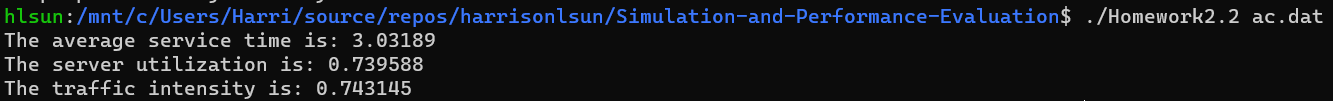
\includegraphics[scale=0.5]{Sections/H2_2.png}\\
The average service time is: 3.03189\\
The server utilization is: 0.739588\\
The traffic intensity is: 0.743145\\\\
